\documentclass[twoside]{book}

% Packages required by doxygen
\usepackage{fixltx2e}
\usepackage{calc}
\usepackage{doxygen}
\usepackage[export]{adjustbox} % also loads graphicx
\usepackage{graphicx}
\usepackage[utf8]{inputenc}
\usepackage{makeidx}
\usepackage{multicol}
\usepackage{multirow}
\PassOptionsToPackage{warn}{textcomp}
\usepackage{textcomp}
\usepackage[nointegrals]{wasysym}
\usepackage[table]{xcolor}

% Font selection
\usepackage[T1]{fontenc}
\usepackage[scaled=.90]{helvet}
\usepackage{courier}
\usepackage{amssymb}
\usepackage{sectsty}
\renewcommand{\familydefault}{\sfdefault}
\allsectionsfont{%
  \fontseries{bc}\selectfont%
  \color{darkgray}%
}
\renewcommand{\DoxyLabelFont}{%
  \fontseries{bc}\selectfont%
  \color{darkgray}%
}
\newcommand{\+}{\discretionary{\mbox{\scriptsize$\hookleftarrow$}}{}{}}

% Page & text layout
\usepackage{geometry}
\geometry{%
  a4paper,%
  top=2.5cm,%
  bottom=2.5cm,%
  left=2.5cm,%
  right=2.5cm%
}
\tolerance=750
\hfuzz=15pt
\hbadness=750
\setlength{\emergencystretch}{15pt}
\setlength{\parindent}{0cm}
\setlength{\parskip}{3ex plus 2ex minus 2ex}
\makeatletter
\renewcommand{\paragraph}{%
  \@startsection{paragraph}{4}{0ex}{-1.0ex}{1.0ex}{%
    \normalfont\normalsize\bfseries\SS@parafont%
  }%
}
\renewcommand{\subparagraph}{%
  \@startsection{subparagraph}{5}{0ex}{-1.0ex}{1.0ex}{%
    \normalfont\normalsize\bfseries\SS@subparafont%
  }%
}
\makeatother

% Headers & footers
\usepackage{fancyhdr}
\pagestyle{fancyplain}
\fancyhead[LE]{\fancyplain{}{\bfseries\thepage}}
\fancyhead[CE]{\fancyplain{}{}}
\fancyhead[RE]{\fancyplain{}{\bfseries\leftmark}}
\fancyhead[LO]{\fancyplain{}{\bfseries\rightmark}}
\fancyhead[CO]{\fancyplain{}{}}
\fancyhead[RO]{\fancyplain{}{\bfseries\thepage}}
\fancyfoot[LE]{\fancyplain{}{}}
\fancyfoot[CE]{\fancyplain{}{}}
\fancyfoot[RE]{\fancyplain{}{\bfseries\scriptsize Generated by Doxygen }}
\fancyfoot[LO]{\fancyplain{}{\bfseries\scriptsize Generated by Doxygen }}
\fancyfoot[CO]{\fancyplain{}{}}
\fancyfoot[RO]{\fancyplain{}{}}
\renewcommand{\footrulewidth}{0.4pt}
\renewcommand{\chaptermark}[1]{%
  \markboth{#1}{}%
}
\renewcommand{\sectionmark}[1]{%
  \markright{\thesection\ #1}%
}

% Indices & bibliography
\usepackage{natbib}
\usepackage[titles]{tocloft}
\setcounter{tocdepth}{3}
\setcounter{secnumdepth}{5}
\makeindex

% Hyperlinks (required, but should be loaded last)
\usepackage{ifpdf}
\ifpdf
  \usepackage[pdftex,pagebackref=true]{hyperref}
\else
  \usepackage[ps2pdf,pagebackref=true]{hyperref}
\fi
\hypersetup{%
  colorlinks=true,%
  linkcolor=blue,%
  citecolor=blue,%
  unicode%
}

% Custom commands
\newcommand{\clearemptydoublepage}{%
  \newpage{\pagestyle{empty}\cleardoublepage}%
}

\usepackage{caption}
\captionsetup{labelsep=space,justification=centering,font={bf},singlelinecheck=off,skip=4pt,position=top}

%===== C O N T E N T S =====

\begin{document}

% Titlepage & ToC
\hypersetup{pageanchor=false,
             bookmarksnumbered=true,
             pdfencoding=unicode
            }
\pagenumbering{roman}
\begin{titlepage}
\vspace*{7cm}
\begin{center}%
{\Large My Project }\\
\vspace*{1cm}
{\large Generated by Doxygen 1.8.11}\\
\end{center}
\end{titlepage}
\clearemptydoublepage
\tableofcontents
\clearemptydoublepage
\pagenumbering{arabic}
\hypersetup{pageanchor=true}

%--- Begin generated contents ---
\chapter{Compressed\+Stacks.\+cpp}
\label{md_README}
\hypertarget{md_README}{}
The Compressed\+Stacks.\+cpp module/library implements a time-\/space trade-\/off structure for stack\textquotesingle{}s algorithms.

\subsection*{Category of algorithms}

This compressed stack structure works correctly as a normal stack for any problems that read input from a file. However, the running time is optimal when the input would be read sequentially with a classical stack structure. For this reason, the only function implemented in the \hyperlink{class_problem}{Problem} template to solve it (to do a run) is the one presented below in a simplified version. 


\begin{DoxyCode}
\textcolor{keyword}{template} <\textcolor{keyword}{class} T, \textcolor{keyword}{class} D> \textcolor{keywordtype}{void} \hyperlink{class_problem}{Problem<T, D>::run}() \{
  initStack();
  \textcolor{keywordflow}{while} (notEndOfFile()) \{
    D data = readInput(line);
    \textcolor{keywordflow}{while} (notEmptystack() && popCondition(data)) \{
      elt = pop();
      popAction(elt);
    \}
    \textcolor{keywordflow}{if} (pushCondition(data)) \{
      pushAction(data);
      push(data);
    \}
  \}
\}
\end{DoxyCode}


\subsection*{Characterization of a problem}

In the followwing examples, implementations of the \hyperlink{class_problem}{Problem} interface are given.

\subsubsection*{General example \+: {\ttfamily \hyperlink{class_instance}{Instance}$<$T,D$>$}}


\begin{DoxyCode}
\textcolor{preprocessor}{#include <string>}
\textcolor{preprocessor}{#include <vector>}
\textcolor{preprocessor}{#include <memory>}

\textcolor{comment}{// T is the type of the context and D is the type of the input data.}
\textcolor{keyword}{class }\hyperlink{class_instance}{Instance}: \textcolor{keyword}{public} \hyperlink{class_problem}{Problem}<T,D>\{
\textcolor{keyword}{public}:
  \hyperlink{class_instance}{Instance}(std::string filePath) : \hyperlink{class_problem}{Problem}<T, D>(filePath) \{\}
\textcolor{keyword}{private}:
  \textcolor{comment}{// Functions to implement according to the problem and input}
  D readInput(std::vector<std::string> line)\{
    std::cout << \textcolor{stringliteral}{"Implement readInput for your instance"} << std::endl;
    \textcolor{keywordflow}{return} 0;
  \}
  std::shared\_ptr<T> initStack()\{
    std::cout << \textcolor{stringliteral}{"Implement initStack for your instance"} << std::endl;
    std::shared\_ptr<T> context(\textcolor{keyword}{nullptr});
    \textcolor{keywordflow}{return} context;
  \}
  \textcolor{keywordtype}{bool} popCondition(D data)\{
    std::cout << \textcolor{stringliteral}{"Implement mPopCondition for your instance"} << std::endl;
    \textcolor{keywordflow}{return} \textcolor{keyword}{false};
  \}
  \textcolor{keywordtype}{void} popAction(\hyperlink{class_data}{Data<T, D>} elt)\{
    std::cout << \textcolor{stringliteral}{"Implement mPopAction for your instance"} << std::endl;
  \}
  \textcolor{keywordtype}{bool} pushCondition(D data)\{
    std::cout << \textcolor{stringliteral}{"Implement mPushCondition for your instance"} << std::endl;
    \textcolor{keywordflow}{return} \textcolor{keyword}{true};
  \}
  \textcolor{keywordtype}{void} pushAction(\hyperlink{class_data}{Data<T, D>} elt)\{
    std::cout << \textcolor{stringliteral}{"Implement mPushAction for your instance"} << std::endl;
  \}
\};
\end{DoxyCode}


\subsubsection*{Example with {\ttfamily T = int} and {\ttfamily D = int} \+: {\ttfamily \hyperlink{class_instance}{Instance}$<$int,int$>$}}

The context is initialized at 0. The data (in cvs format) is read as a pair of string such that the first string is the data and the second is used to update the context. While the context is more than 0, the stack is poped and the context decreased by 1. If the data is more than 0 then it is pushed. 
\begin{DoxyCode}
\textcolor{keyword}{class }\hyperlink{class_instance}{Instance} : \textcolor{keyword}{public} \hyperlink{class_problem}{Problem}<int, int> \{
\textcolor{keyword}{public}:
  \hyperlink{class_instance}{Instance}(std::string filePath) : \hyperlink{class_problem}{Problem}<int, int>(filePath) \{\}

\textcolor{keyword}{private}:
  \textcolor{comment}{// Functions to run the stack}
  \textcolor{keywordtype}{int} readInput(std::vector<std::string> line) \{
    \textcolor{keywordtype}{int} value = std::stoi(line[0]);
    setContext(std::stoi(line[1]));
    \textcolor{keywordflow}{return} value;
  \}
  std::shared\_ptr<int> initStack() \{
    std::shared\_ptr<int> context(\textcolor{keyword}{new} \textcolor{keywordtype}{int}(0));
    \textcolor{keywordflow}{return} context;
  \}
  \textcolor{keywordtype}{bool} popCondition(\textcolor{keywordtype}{int} data) \{
    \textcolor{keywordflow}{if} ((getContext() > 0)) \{
      \textcolor{keywordflow}{return} \textcolor{keyword}{true};
    \}
    \textcolor{keywordflow}{return} \textcolor{keyword}{false};
  \}
  \textcolor{keywordtype}{void} popAction(\hyperlink{class_data}{Data<int, int>} elt) \{
    std::cout << elt.toString() << \textcolor{stringliteral}{" <<<< Pop!"} << std::endl;
    setContext(getContext() - 1);
  \}
  \textcolor{keywordtype}{bool} pushCondition(\textcolor{keywordtype}{int} data) \{
    \textcolor{keywordflow}{if} (data > 0) \{
      \textcolor{keywordflow}{return} \textcolor{keyword}{true};
    \}
    \textcolor{keywordflow}{return} \textcolor{keyword}{false};
  \}
  \textcolor{keywordtype}{void} pushAction(\hyperlink{class_data}{Data<int, int>} elt) \{
    std::cout << \textcolor{stringliteral}{"Push >>>> "} << elt.toString() << std::endl;
  \}
\};
\end{DoxyCode}


\subsection*{How to run your problem}

Suppose the class \hyperlink{class_instance}{Instance} implement the interface Problem$<$\+T,\+D$>$ (as in some examples above). You can run an instance of your problem described in the input located at {\itshape filepath}. The last command just print an output in th console of your compressed stack after the run.


\begin{DoxyCode}
\hyperlink{class_instance}{Instance} stack(filePath);
stack.run();
stack.println();
\end{DoxyCode}
 
\chapter{Hierarchical Index}
\section{Class Hierarchy}
This inheritance list is sorted roughly, but not completely, alphabetically\+:\begin{DoxyCompactList}
\item \contentsline{section}{Buffer$<$ T, D $>$}{\pageref{class_buffer}}{}
\item \contentsline{section}{Component$<$ T, D $>$}{\pageref{class_component}}{}
\item \contentsline{section}{create\+Test\+Input}{\pageref{classcreate_test_input}}{}
\item \contentsline{section}{Data$<$ T, D $>$}{\pageref{class_data}}{}
\item \contentsline{section}{empty\+Context}{\pageref{classempty_context}}{}
\item \contentsline{section}{Point2D}{\pageref{class_point2_d}}{}
\item \contentsline{section}{Problem$<$ T, D $>$}{\pageref{class_problem}}{}
\begin{DoxyCompactList}
\item \contentsline{section}{Compare\+Stacks$<$ T, D $>$}{\pageref{class_compare_stacks}}{}
\end{DoxyCompactList}
\item \contentsline{section}{Problem$<$ empty\+Context, Point2D $>$}{\pageref{class_problem}}{}
\begin{DoxyCompactList}
\item \contentsline{section}{Compare\+Stacks$<$ empty\+Context, Point2D $>$}{\pageref{class_compare_stacks}}{}
\begin{DoxyCompactList}
\item \contentsline{section}{comparison\+Convex\+Hull}{\pageref{classcomparison_convex_hull}}{}
\end{DoxyCompactList}
\item \contentsline{section}{convex\+Hull}{\pageref{classconvex_hull}}{}
\end{DoxyCompactList}
\item \contentsline{section}{Problem$<$ int, int $>$}{\pageref{class_problem}}{}
\begin{DoxyCompactList}
\item \contentsline{section}{Compare\+Stacks$<$ int, int $>$}{\pageref{class_compare_stacks}}{}
\begin{DoxyCompactList}
\item \contentsline{section}{Comparison}{\pageref{class_comparison}}{}
\end{DoxyCompactList}
\item \contentsline{section}{Instance}{\pageref{class_instance}}{}
\end{DoxyCompactList}
\item \contentsline{section}{Signature$<$ T, D $>$}{\pageref{class_signature}}{}
\item \contentsline{section}{Stack$<$ T, D $>$}{\pageref{class_stack}}{}
\begin{DoxyCompactList}
\item \contentsline{section}{Compressed\+Stack$<$ T, D $>$}{\pageref{class_compressed_stack}}{}
\item \contentsline{section}{Normal\+Stack$<$ T, D $>$}{\pageref{class_normal_stack}}{}
\end{DoxyCompactList}
\end{DoxyCompactList}

\chapter{Class Index}
\section{Class List}
Here are the classes, structs, unions and interfaces with brief descriptions\+:\begin{DoxyCompactList}
\item\contentsline{section}{\hyperlink{class_buffer}{Buffer$<$ T, D $>$} }{\pageref{class_buffer}}{}
\item\contentsline{section}{\hyperlink{class_compare_stacks}{Compare\+Stacks$<$ T, D $>$} }{\pageref{class_compare_stacks}}{}
\item\contentsline{section}{\hyperlink{class_comparison}{Comparison} }{\pageref{class_comparison}}{}
\item\contentsline{section}{\hyperlink{classcomparison_convex_hull}{comparison\+Convex\+Hull} }{\pageref{classcomparison_convex_hull}}{}
\item\contentsline{section}{\hyperlink{class_component}{Component$<$ T, D $>$} }{\pageref{class_component}}{}
\item\contentsline{section}{\hyperlink{class_compressed_stack}{Compressed\+Stack$<$ T, D $>$} }{\pageref{class_compressed_stack}}{}
\item\contentsline{section}{\hyperlink{classconvex_hull}{convex\+Hull} }{\pageref{classconvex_hull}}{}
\item\contentsline{section}{\hyperlink{classcreate_test_input}{create\+Test\+Input} }{\pageref{classcreate_test_input}}{}
\item\contentsline{section}{\hyperlink{class_data}{Data$<$ T, D $>$} }{\pageref{class_data}}{}
\item\contentsline{section}{\hyperlink{classempty_context}{empty\+Context} }{\pageref{classempty_context}}{}
\item\contentsline{section}{\hyperlink{class_instance}{Instance} }{\pageref{class_instance}}{}
\item\contentsline{section}{\hyperlink{class_normal_stack}{Normal\+Stack$<$ T, D $>$} }{\pageref{class_normal_stack}}{}
\item\contentsline{section}{\hyperlink{class_point2_d}{Point2D} }{\pageref{class_point2_d}}{}
\item\contentsline{section}{\hyperlink{class_problem}{Problem$<$ T, D $>$} }{\pageref{class_problem}}{}
\item\contentsline{section}{\hyperlink{class_signature}{Signature$<$ T, D $>$} }{\pageref{class_signature}}{}
\item\contentsline{section}{\hyperlink{class_stack}{Stack$<$ T, D $>$} }{\pageref{class_stack}}{}
\end{DoxyCompactList}

\chapter{Class Documentation}
\hypertarget{class_buffer}{}\section{Buffer$<$ T, D $>$ Class Template Reference}
\label{class_buffer}\index{Buffer$<$ T, D $>$@{Buffer$<$ T, D $>$}}


Collaboration diagram for Buffer$<$ T, D $>$\+:
\nopagebreak
\begin{figure}[H]
\begin{center}
\leavevmode
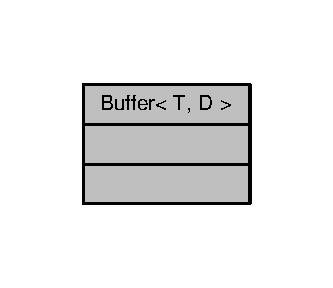
\includegraphics[width=160pt]{class_buffer__coll__graph}
\end{center}
\end{figure}
\subsection*{Friends}
\begin{DoxyCompactItemize}
\item 
class {\bfseries Compressed\+Stack$<$ T, D $>$}\hypertarget{class_buffer_a0bc563c952d4b72ba232305ab7717bd9}{}\label{class_buffer_a0bc563c952d4b72ba232305ab7717bd9}

\item 
class {\bfseries Normal\+Stack$<$ T, D $>$}\hypertarget{class_buffer_a3448f5e6d9366f8729b55e62587568ca}{}\label{class_buffer_a3448f5e6d9366f8729b55e62587568ca}

\item 
class {\bfseries Signature$<$ T, D $>$}\hypertarget{class_buffer_a3bdacd57a94b060eb49095b91e06e01e}{}\label{class_buffer_a3bdacd57a94b060eb49095b91e06e01e}

\item 
class {\bfseries Component$<$ T, D $>$}\hypertarget{class_buffer_a843c2f068a1ab99ce6c9c0e2cc3946c5}{}\label{class_buffer_a843c2f068a1ab99ce6c9c0e2cc3946c5}

\end{DoxyCompactItemize}


The documentation for this class was generated from the following file\+:\begin{DoxyCompactItemize}
\item 
include/buffer.\+hpp\end{DoxyCompactItemize}

\hypertarget{class_compare_stacks}{}\section{Compare\+Stacks$<$ T, D $>$ Class Template Reference}
\label{class_compare_stacks}\index{Compare\+Stacks$<$ T, D $>$@{Compare\+Stacks$<$ T, D $>$}}


Inheritance diagram for Compare\+Stacks$<$ T, D $>$\+:
\nopagebreak
\begin{figure}[H]
\begin{center}
\leavevmode
\includegraphics[height=550pt]{class_compare_stacks__inherit__graph}
\end{center}
\end{figure}


Collaboration diagram for Compare\+Stacks$<$ T, D $>$\+:
\nopagebreak
\begin{figure}[H]
\begin{center}
\leavevmode
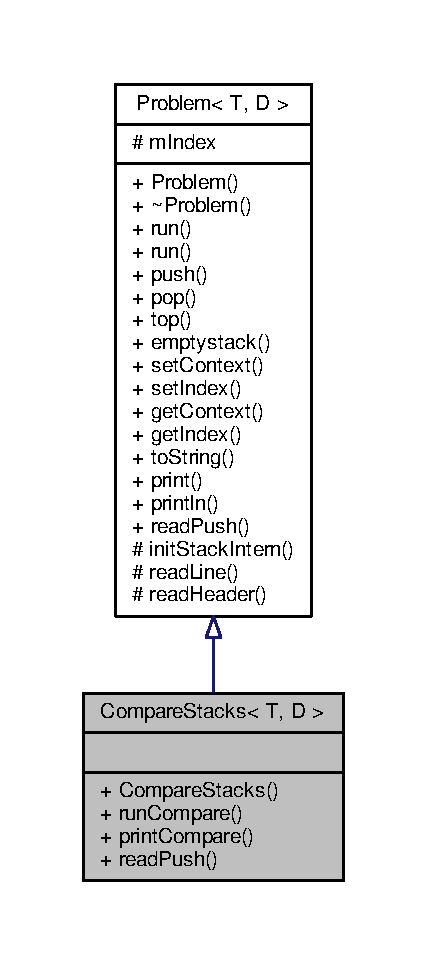
\includegraphics[width=205pt]{class_compare_stacks__coll__graph}
\end{center}
\end{figure}
\subsection*{Public Member Functions}
\begin{DoxyCompactItemize}
\item 
{\bfseries Compare\+Stacks} (std\+::string file\+Name)\hypertarget{class_compare_stacks_a0f3c2b21705805d2e80f528bbc3bcb3f}{}\label{class_compare_stacks_a0f3c2b21705805d2e80f528bbc3bcb3f}

\item 
void {\bfseries run\+Compare} (int buffer=0)\hypertarget{class_compare_stacks_ae90c5d2cc73db90fa62a918e939a2a9d}{}\label{class_compare_stacks_ae90c5d2cc73db90fa62a918e939a2a9d}

\item 
void {\bfseries print\+Compare} ()\hypertarget{class_compare_stacks_a9b1bcc007486170cc82167b6f609b37d}{}\label{class_compare_stacks_a9b1bcc007486170cc82167b6f609b37d}

\item 
void {\bfseries read\+Push} (int iter=1)\hypertarget{class_compare_stacks_ad4a4749ec1085d57d04165e1ec92efe5}{}\label{class_compare_stacks_ad4a4749ec1085d57d04165e1ec92efe5}

\end{DoxyCompactItemize}
\subsection*{Additional Inherited Members}


The documentation for this class was generated from the following file\+:\begin{DoxyCompactItemize}
\item 
include/compare.\+hpp\end{DoxyCompactItemize}

\hypertarget{class_comparison}{}\section{Comparison Class Reference}
\label{class_comparison}\index{Comparison@{Comparison}}


Inheritance diagram for Comparison\+:
\nopagebreak
\begin{figure}[H]
\begin{center}
\leavevmode
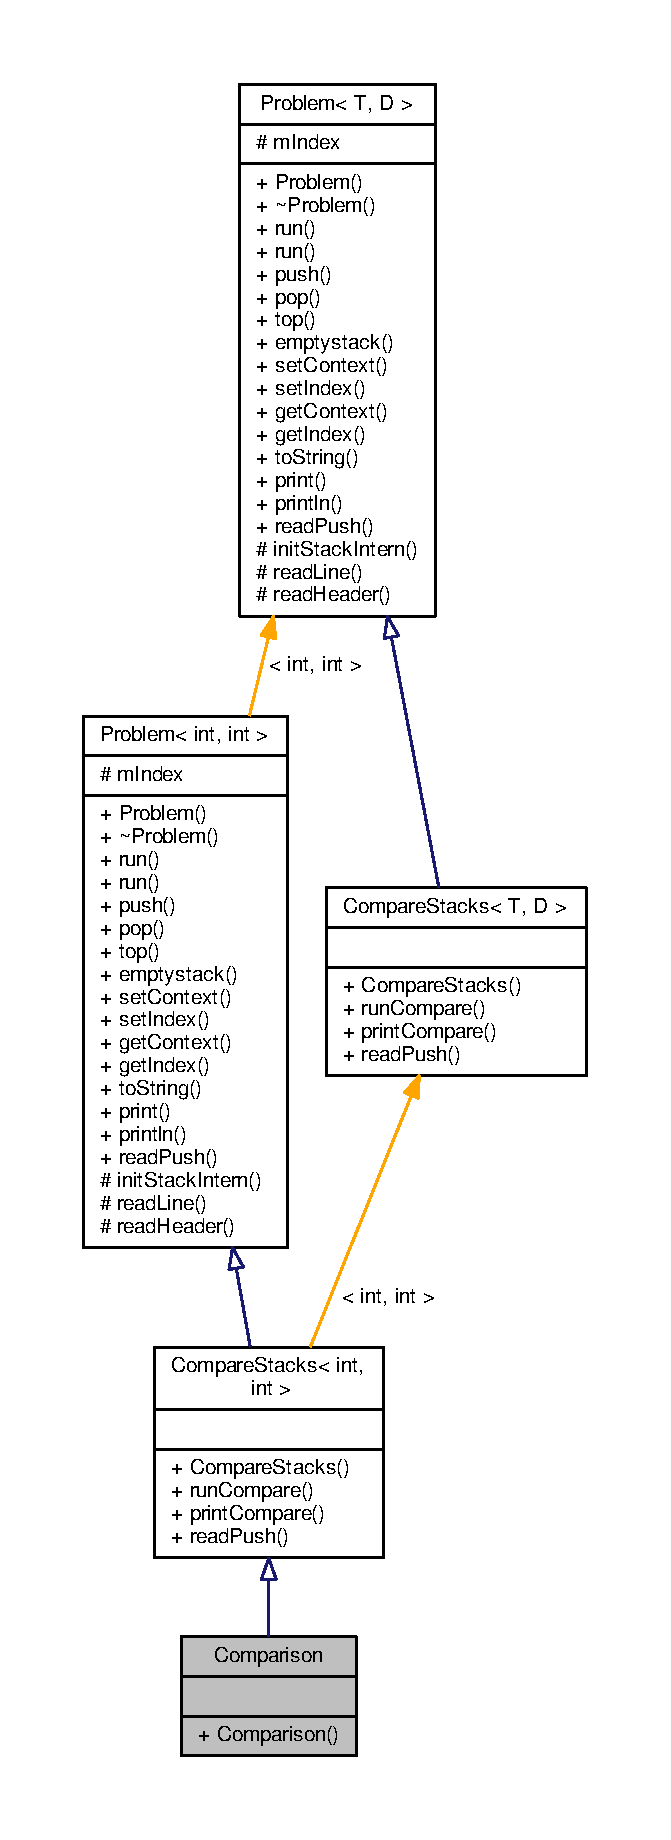
\includegraphics[height=550pt]{class_comparison__inherit__graph}
\end{center}
\end{figure}


Collaboration diagram for Comparison\+:
\nopagebreak
\begin{figure}[H]
\begin{center}
\leavevmode
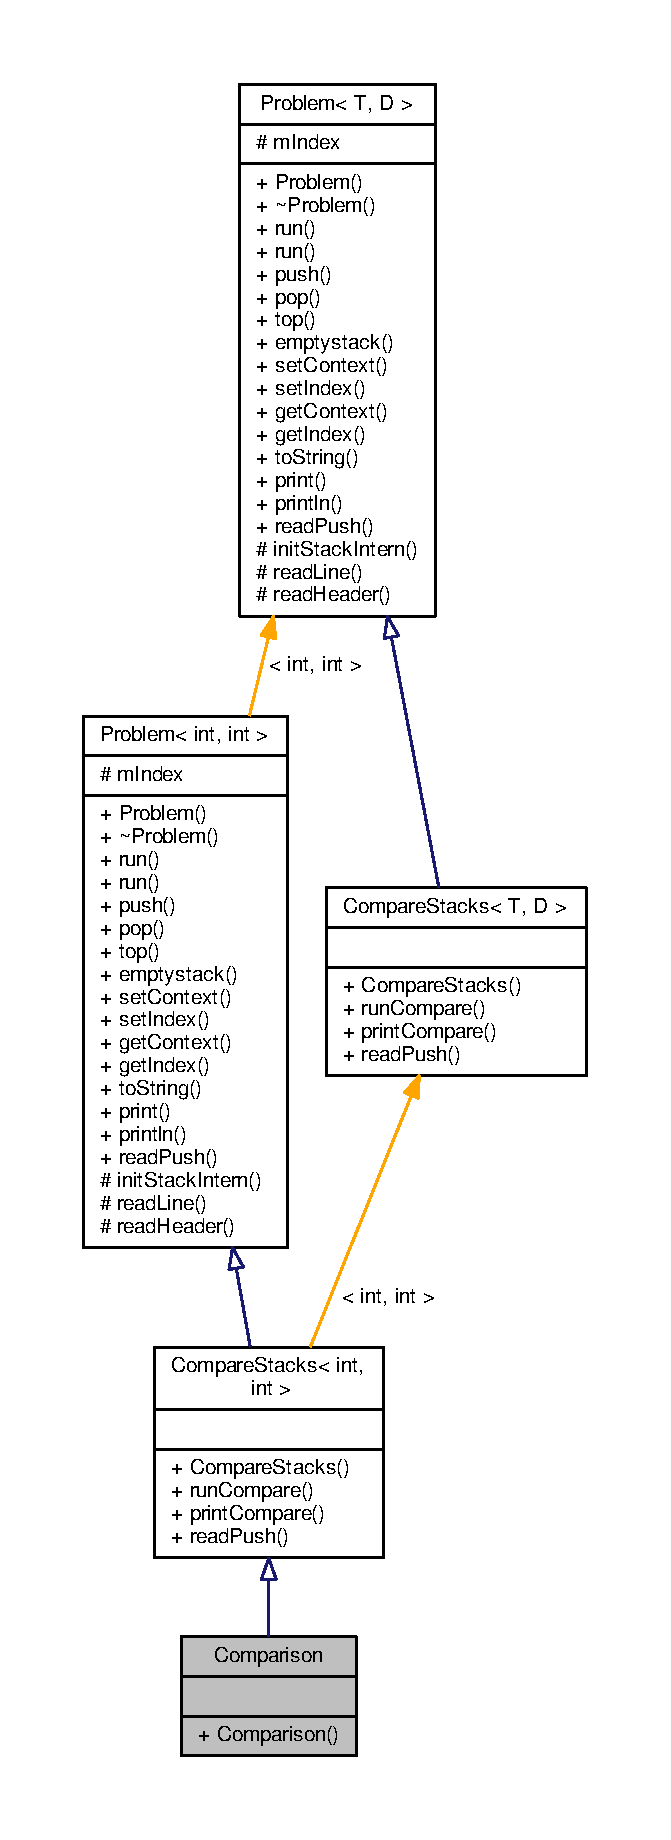
\includegraphics[height=550pt]{class_comparison__coll__graph}
\end{center}
\end{figure}
\subsection*{Public Member Functions}
\begin{DoxyCompactItemize}
\item 
{\bfseries Comparison} (std\+::string file\+Path)\hypertarget{class_comparison_a24fad3f45a7c7c6bd53aaadf93fe2043}{}\label{class_comparison_a24fad3f45a7c7c6bd53aaadf93fe2043}

\end{DoxyCompactItemize}
\subsection*{Additional Inherited Members}


The documentation for this class was generated from the following file\+:\begin{DoxyCompactItemize}
\item 
src/main.\+cpp\end{DoxyCompactItemize}

\hypertarget{classcomparison_convex_hull}{}\section{comparison\+Convex\+Hull Class Reference}
\label{classcomparison_convex_hull}\index{comparison\+Convex\+Hull@{comparison\+Convex\+Hull}}


Inheritance diagram for comparison\+Convex\+Hull\+:
\nopagebreak
\begin{figure}[H]
\begin{center}
\leavevmode
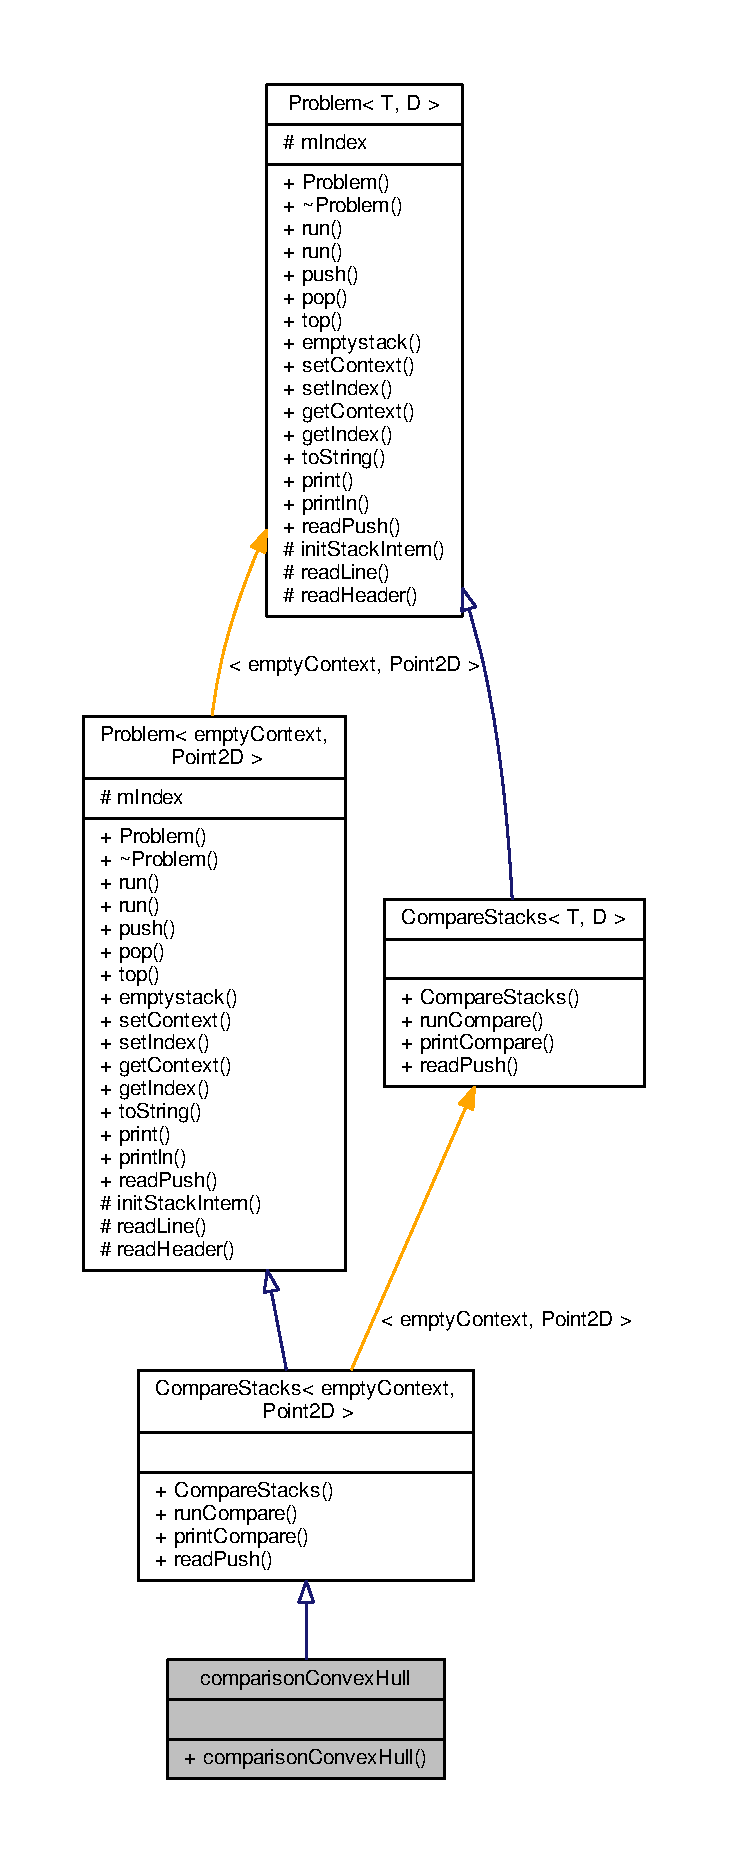
\includegraphics[height=550pt]{classcomparison_convex_hull__inherit__graph}
\end{center}
\end{figure}


Collaboration diagram for comparison\+Convex\+Hull\+:
\nopagebreak
\begin{figure}[H]
\begin{center}
\leavevmode
\includegraphics[height=550pt]{classcomparison_convex_hull__coll__graph}
\end{center}
\end{figure}
\subsection*{Public Member Functions}
\begin{DoxyCompactItemize}
\item 
{\bfseries comparison\+Convex\+Hull} (std\+::string file\+Path)\hypertarget{classcomparison_convex_hull_adbb31faac10cca011853284d8e7b021a}{}\label{classcomparison_convex_hull_adbb31faac10cca011853284d8e7b021a}

\end{DoxyCompactItemize}
\subsection*{Additional Inherited Members}


The documentation for this class was generated from the following files\+:\begin{DoxyCompactItemize}
\item 
include/convex\+Hull.\+hpp\item 
src/convex\+Hull.\+cpp\end{DoxyCompactItemize}

\hypertarget{class_component}{}\section{Component$<$ T, D $>$ Class Template Reference}
\label{class_component}\index{Component$<$ T, D $>$@{Component$<$ T, D $>$}}


Collaboration diagram for Component$<$ T, D $>$\+:
\nopagebreak
\begin{figure}[H]
\begin{center}
\leavevmode
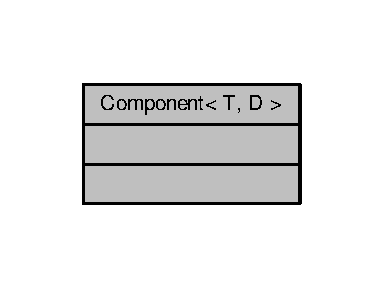
\includegraphics[width=184pt]{class_component__coll__graph}
\end{center}
\end{figure}
\subsection*{Friends}
\begin{DoxyCompactItemize}
\item 
class {\bfseries Compressed\+Stack$<$ T, D $>$}\hypertarget{class_component_a0bc563c952d4b72ba232305ab7717bd9}{}\label{class_component_a0bc563c952d4b72ba232305ab7717bd9}

\end{DoxyCompactItemize}


The documentation for this class was generated from the following files\+:\begin{DoxyCompactItemize}
\item 
include/buffer.\+hpp\item 
include/component.\+hpp\end{DoxyCompactItemize}

\hypertarget{class_compressed_stack}{}\section{Compressed\+Stack$<$ T, D $>$ Class Template Reference}
\label{class_compressed_stack}\index{Compressed\+Stack$<$ T, D $>$@{Compressed\+Stack$<$ T, D $>$}}


Inheritance diagram for Compressed\+Stack$<$ T, D $>$\+:
\nopagebreak
\begin{figure}[H]
\begin{center}
\leavevmode
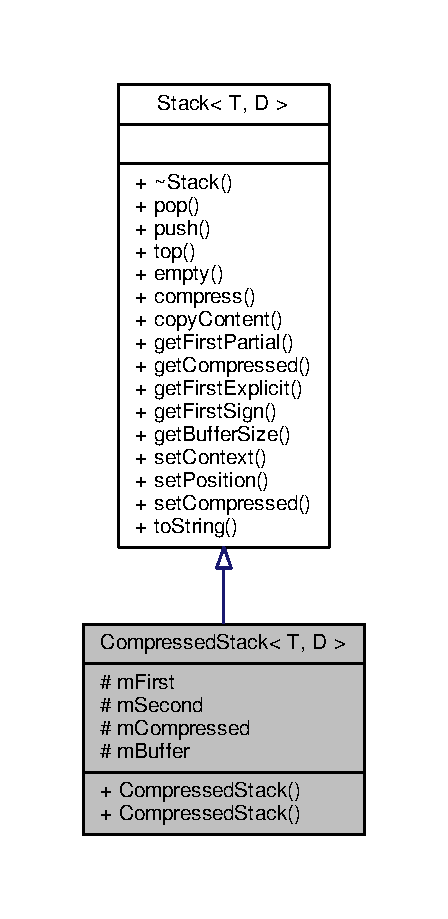
\includegraphics[width=215pt]{class_compressed_stack__inherit__graph}
\end{center}
\end{figure}


Collaboration diagram for Compressed\+Stack$<$ T, D $>$\+:
\nopagebreak
\begin{figure}[H]
\begin{center}
\leavevmode
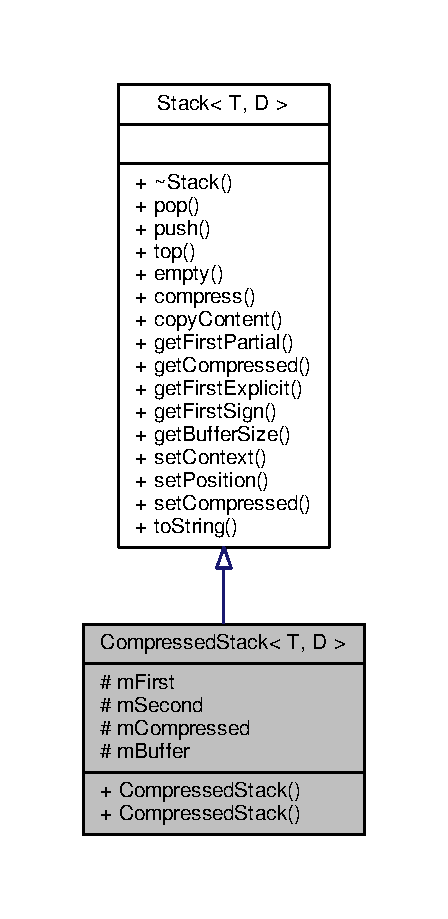
\includegraphics[width=215pt]{class_compressed_stack__coll__graph}
\end{center}
\end{figure}
\subsection*{Public Member Functions}
\begin{DoxyCompactItemize}
\item 
{\bfseries Compressed\+Stack} (int size, int space, int buffer, std\+::shared\+\_\+ptr$<$ T $>$ context, std\+::streampos position=std\+::streampos(0))\hypertarget{class_compressed_stack_adbfd81811e7061deccacbbe2ec1709ec}{}\label{class_compressed_stack_adbfd81811e7061deccacbbe2ec1709ec}

\item 
{\bfseries Compressed\+Stack} (int size, int space, int buffer, const \hyperlink{class_signature}{Signature}$<$ T, D $>$ \&sign)\hypertarget{class_compressed_stack_aa51942713c62d541ddcce32e433642e4}{}\label{class_compressed_stack_aa51942713c62d541ddcce32e433642e4}

\end{DoxyCompactItemize}
\subsection*{Protected Attributes}
\begin{DoxyCompactItemize}
\item 
\hyperlink{class_component}{Component}$<$ T, D $>$ {\bfseries m\+First}\hypertarget{class_compressed_stack_a01b36c057eea8081a803aa4aa2eaf9f2}{}\label{class_compressed_stack_a01b36c057eea8081a803aa4aa2eaf9f2}

\item 
\hyperlink{class_component}{Component}$<$ T, D $>$ {\bfseries m\+Second}\hypertarget{class_compressed_stack_ae7318db14913195490d6dde2323ad1bf}{}\label{class_compressed_stack_ae7318db14913195490d6dde2323ad1bf}

\item 
Block$<$ T, D $>$ {\bfseries m\+Compressed}\hypertarget{class_compressed_stack_a67f78c7cdcac6d2e9339c9c4b5f3b60c}{}\label{class_compressed_stack_a67f78c7cdcac6d2e9339c9c4b5f3b60c}

\item 
\hyperlink{class_buffer}{Buffer}$<$ T, D $>$ {\bfseries m\+Buffer}\hypertarget{class_compressed_stack_a6ea67dc13c6b584d2257f18eefcc158f}{}\label{class_compressed_stack_a6ea67dc13c6b584d2257f18eefcc158f}

\end{DoxyCompactItemize}
\subsection*{Friends}
\begin{DoxyCompactItemize}
\item 
class {\bfseries Problem$<$ T, D $>$}\hypertarget{class_compressed_stack_a49d2c5c1103bce3a8ba02241be7f15c0}{}\label{class_compressed_stack_a49d2c5c1103bce3a8ba02241be7f15c0}

\end{DoxyCompactItemize}


The documentation for this class was generated from the following files\+:\begin{DoxyCompactItemize}
\item 
include/buffer.\+hpp\item 
include/compressed\+Stack.\+hpp\end{DoxyCompactItemize}

\hypertarget{classconvex_hull}{}\section{convex\+Hull Class Reference}
\label{classconvex_hull}\index{convex\+Hull@{convex\+Hull}}


Inheritance diagram for convex\+Hull\+:
\nopagebreak
\begin{figure}[H]
\begin{center}
\leavevmode
\includegraphics[height=550pt]{classconvex_hull__inherit__graph}
\end{center}
\end{figure}


Collaboration diagram for convex\+Hull\+:
\nopagebreak
\begin{figure}[H]
\begin{center}
\leavevmode
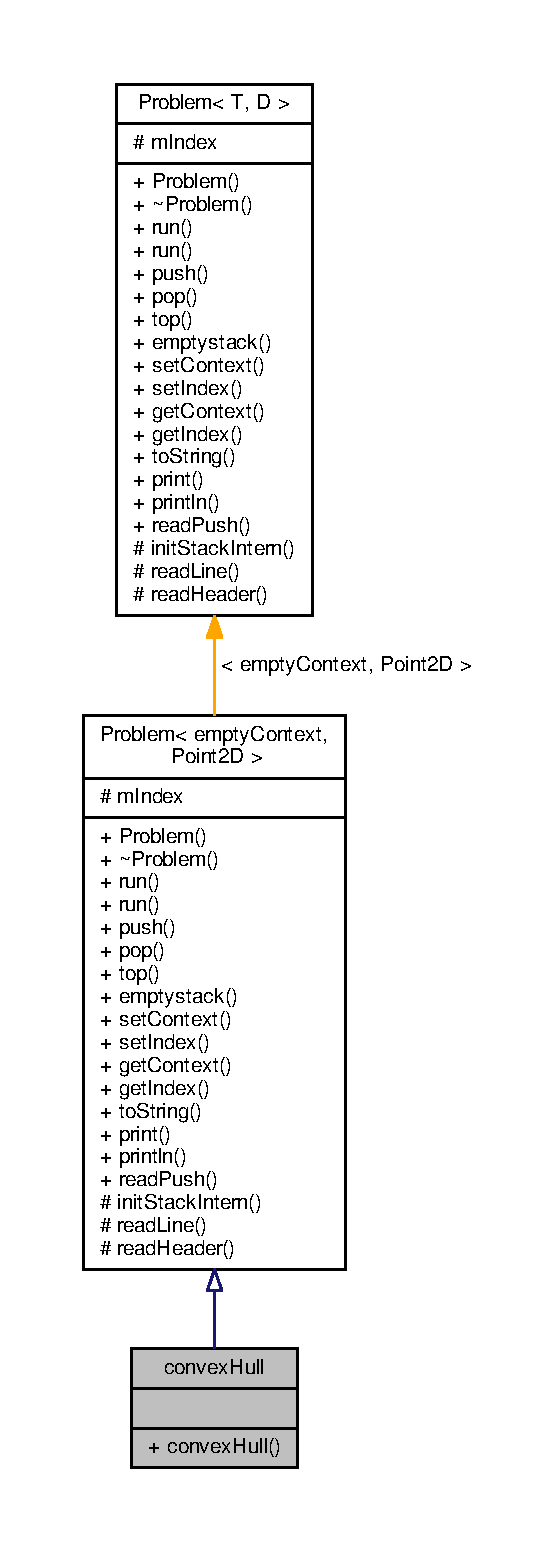
\includegraphics[height=550pt]{classconvex_hull__coll__graph}
\end{center}
\end{figure}
\subsection*{Public Member Functions}
\begin{DoxyCompactItemize}
\item 
{\bfseries convex\+Hull} (std\+::string file\+Path)\hypertarget{classconvex_hull_a36e1e32ed7c3c3b183cd2ea2d35b16b1}{}\label{classconvex_hull_a36e1e32ed7c3c3b183cd2ea2d35b16b1}

\end{DoxyCompactItemize}
\subsection*{Additional Inherited Members}


The documentation for this class was generated from the following files\+:\begin{DoxyCompactItemize}
\item 
include/convex\+Hull.\+hpp\item 
src/convex\+Hull.\+cpp\end{DoxyCompactItemize}

\hypertarget{classcreate_test_input}{}\section{create\+Test\+Input Class Reference}
\label{classcreate_test_input}\index{create\+Test\+Input@{create\+Test\+Input}}


Collaboration diagram for create\+Test\+Input\+:
\nopagebreak
\begin{figure}[H]
\begin{center}
\leavevmode
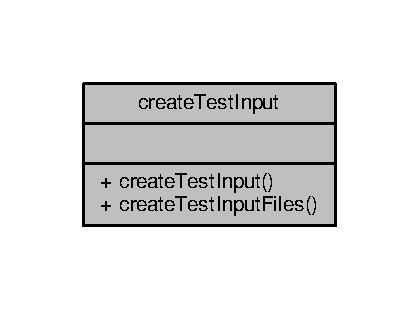
\includegraphics[width=201pt]{classcreate_test_input__coll__graph}
\end{center}
\end{figure}
\subsection*{Public Member Functions}
\begin{DoxyCompactItemize}
\item 
void {\bfseries create\+Test\+Input\+Files} (int code, int stacktype, std\+::string file\+Name, int n, int p, int min=0, int max=100, double prob=0)\hypertarget{classcreate_test_input_a28ea5139369c516837187beaa44b141c}{}\label{classcreate_test_input_a28ea5139369c516837187beaa44b141c}

\end{DoxyCompactItemize}


The documentation for this class was generated from the following files\+:\begin{DoxyCompactItemize}
\item 
include/create\+Test\+Input.\+hpp\item 
src/create\+Test\+Input.\+cpp\end{DoxyCompactItemize}

\hypertarget{class_data}{}\section{Data$<$ T, D $>$ Class Template Reference}
\label{class_data}\index{Data$<$ T, D $>$@{Data$<$ T, D $>$}}


Collaboration diagram for Data$<$ T, D $>$\+:
\nopagebreak
\begin{figure}[H]
\begin{center}
\leavevmode
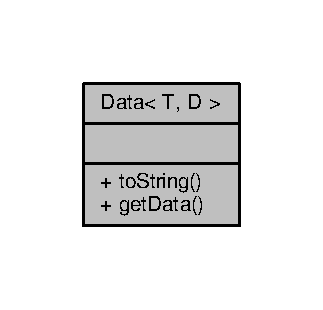
\includegraphics[width=155pt]{class_data__coll__graph}
\end{center}
\end{figure}
\subsection*{Public Member Functions}
\begin{DoxyCompactItemize}
\item 
std\+::string {\bfseries to\+String} ()\hypertarget{class_data_a8f7071b4c9d15f57af376b981a6e3c12}{}\label{class_data_a8f7071b4c9d15f57af376b981a6e3c12}

\item 
D {\bfseries get\+Data} ()\hypertarget{class_data_a8998e5093d23c19b585ad829e65e3b8b}{}\label{class_data_a8998e5093d23c19b585ad829e65e3b8b}

\end{DoxyCompactItemize}
\subsection*{Friends}
\begin{DoxyCompactItemize}
\item 
class {\bfseries Component$<$ T, D $>$}\hypertarget{class_data_a843c2f068a1ab99ce6c9c0e2cc3946c5}{}\label{class_data_a843c2f068a1ab99ce6c9c0e2cc3946c5}

\item 
class {\bfseries Compressed\+Stack$<$ T, D $>$}\hypertarget{class_data_a0bc563c952d4b72ba232305ab7717bd9}{}\label{class_data_a0bc563c952d4b72ba232305ab7717bd9}

\item 
class {\bfseries Problem$<$ T, D $>$}\hypertarget{class_data_a49d2c5c1103bce3a8ba02241be7f15c0}{}\label{class_data_a49d2c5c1103bce3a8ba02241be7f15c0}

\item 
class {\bfseries Compare\+Stacks$<$ T, D $>$}\hypertarget{class_data_aad0b6ceccdc6599793a7e2e5798b59ad}{}\label{class_data_aad0b6ceccdc6599793a7e2e5798b59ad}

\item 
class {\bfseries Comparison}\hypertarget{class_data_aef3aa9a02bb7e4bcae2ebd8975a9206d}{}\label{class_data_aef3aa9a02bb7e4bcae2ebd8975a9206d}

\end{DoxyCompactItemize}


The documentation for this class was generated from the following file\+:\begin{DoxyCompactItemize}
\item 
include/data.\+hpp\end{DoxyCompactItemize}

\hypertarget{classempty_context}{}\section{empty\+Context Class Reference}
\label{classempty_context}\index{empty\+Context@{empty\+Context}}


Collaboration diagram for empty\+Context\+:
\nopagebreak
\begin{figure}[H]
\begin{center}
\leavevmode
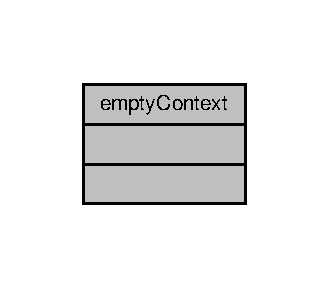
\includegraphics[width=158pt]{classempty_context__coll__graph}
\end{center}
\end{figure}


The documentation for this class was generated from the following file\+:\begin{DoxyCompactItemize}
\item 
include/convex\+Hull.\+hpp\end{DoxyCompactItemize}

\hypertarget{class_instance}{}\section{Instance Class Reference}
\label{class_instance}\index{Instance@{Instance}}


Inheritance diagram for Instance\+:
\nopagebreak
\begin{figure}[H]
\begin{center}
\leavevmode
\includegraphics[height=550pt]{class_instance__inherit__graph}
\end{center}
\end{figure}


Collaboration diagram for Instance\+:
\nopagebreak
\begin{figure}[H]
\begin{center}
\leavevmode
\includegraphics[height=550pt]{class_instance__coll__graph}
\end{center}
\end{figure}
\subsection*{Public Member Functions}
\begin{DoxyCompactItemize}
\item 
{\bfseries Instance} (std\+::string file\+Path)\hypertarget{class_instance_a4481e14389cf698ecd6f48ca1c86c60a}{}\label{class_instance_a4481e14389cf698ecd6f48ca1c86c60a}

\end{DoxyCompactItemize}
\subsection*{Additional Inherited Members}


The documentation for this class was generated from the following file\+:\begin{DoxyCompactItemize}
\item 
src/main.\+cpp\end{DoxyCompactItemize}

\hypertarget{class_normal_stack}{}\section{Normal\+Stack$<$ T, D $>$ Class Template Reference}
\label{class_normal_stack}\index{Normal\+Stack$<$ T, D $>$@{Normal\+Stack$<$ T, D $>$}}


Inheritance diagram for Normal\+Stack$<$ T, D $>$\+:
\nopagebreak
\begin{figure}[H]
\begin{center}
\leavevmode
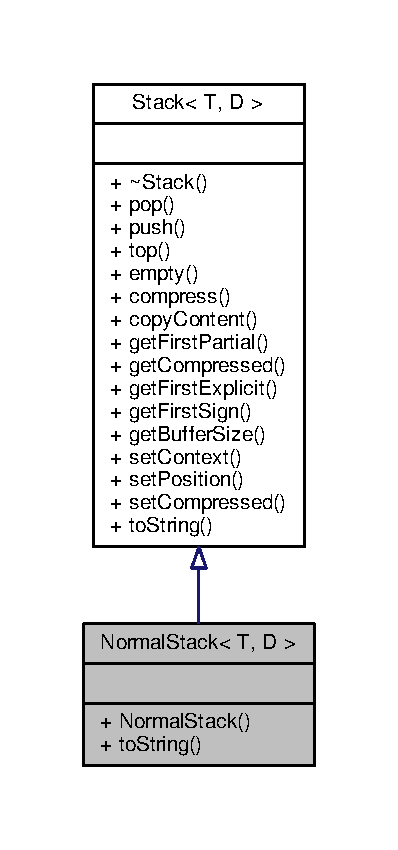
\includegraphics[width=191pt]{class_normal_stack__inherit__graph}
\end{center}
\end{figure}


Collaboration diagram for Normal\+Stack$<$ T, D $>$\+:
\nopagebreak
\begin{figure}[H]
\begin{center}
\leavevmode
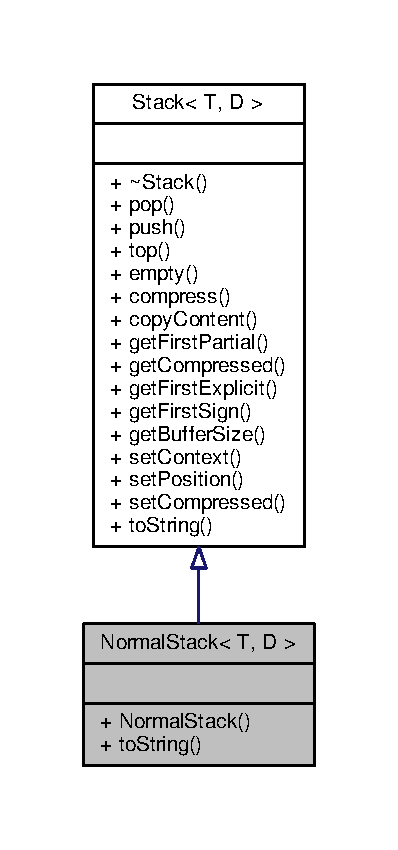
\includegraphics[width=191pt]{class_normal_stack__coll__graph}
\end{center}
\end{figure}
\subsection*{Public Member Functions}
\begin{DoxyCompactItemize}
\item 
std\+::string {\bfseries to\+String} ()\hypertarget{class_normal_stack_afdfa737b000d756b1edc7bb077d79137}{}\label{class_normal_stack_afdfa737b000d756b1edc7bb077d79137}

\end{DoxyCompactItemize}
\subsection*{Friends}
\begin{DoxyCompactItemize}
\item 
class {\bfseries Problem$<$ T, D $>$}\hypertarget{class_normal_stack_a49d2c5c1103bce3a8ba02241be7f15c0}{}\label{class_normal_stack_a49d2c5c1103bce3a8ba02241be7f15c0}

\item 
class {\bfseries Compare\+Stacks$<$ T, D $>$}\hypertarget{class_normal_stack_aad0b6ceccdc6599793a7e2e5798b59ad}{}\label{class_normal_stack_aad0b6ceccdc6599793a7e2e5798b59ad}

\item 
class {\bfseries Comparison}\hypertarget{class_normal_stack_aef3aa9a02bb7e4bcae2ebd8975a9206d}{}\label{class_normal_stack_aef3aa9a02bb7e4bcae2ebd8975a9206d}

\end{DoxyCompactItemize}


The documentation for this class was generated from the following files\+:\begin{DoxyCompactItemize}
\item 
include/buffer.\+hpp\item 
include/normal\+Stack.\+hpp\end{DoxyCompactItemize}

\hypertarget{class_point2_d}{}\section{Point2D Class Reference}
\label{class_point2_d}\index{Point2D@{Point2D}}


Collaboration diagram for Point2D\+:
\nopagebreak
\begin{figure}[H]
\begin{center}
\leavevmode
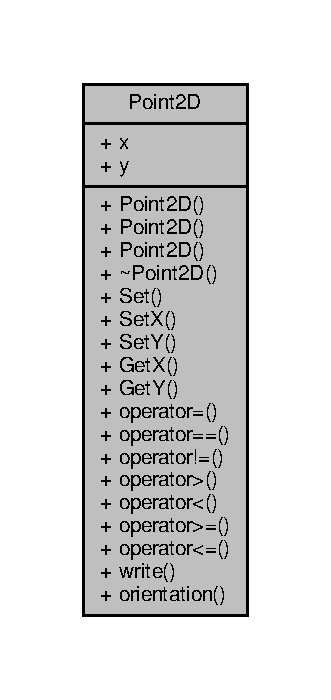
\includegraphics[width=159pt]{class_point2_d__coll__graph}
\end{center}
\end{figure}
\subsection*{Public Member Functions}
\begin{DoxyCompactItemize}
\item 
{\bfseries Point2D} (double x, double y)\hypertarget{class_point2_d_ac9d8daeb64c1e93325c7868d42da6e44}{}\label{class_point2_d_ac9d8daeb64c1e93325c7868d42da6e44}

\item 
{\bfseries Point2D} (const \hyperlink{class_point2_d}{Point2D} \&other)\hypertarget{class_point2_d_a0c7330a979e83d7de8253089d201cdd3}{}\label{class_point2_d_a0c7330a979e83d7de8253089d201cdd3}

\item 
void {\bfseries Set} (const double x, const double y)\hypertarget{class_point2_d_a9b256ee317e41ab97d0214ec0e9ed6ad}{}\label{class_point2_d_a9b256ee317e41ab97d0214ec0e9ed6ad}

\item 
void {\bfseries SetX} (double x)\hypertarget{class_point2_d_ae2c20141053387e138970b8b3585e9a2}{}\label{class_point2_d_ae2c20141053387e138970b8b3585e9a2}

\item 
void {\bfseries SetY} (double y)\hypertarget{class_point2_d_a446a5d31f7dd7ed665381fc466c707ff}{}\label{class_point2_d_a446a5d31f7dd7ed665381fc466c707ff}

\item 
double {\bfseries GetX} () const \hypertarget{class_point2_d_aee760e0f9996f2bc71fa873c57871e0a}{}\label{class_point2_d_aee760e0f9996f2bc71fa873c57871e0a}

\item 
double {\bfseries GetY} () const \hypertarget{class_point2_d_ac30d12c0468c1f81b6939edd3941ae7d}{}\label{class_point2_d_ac30d12c0468c1f81b6939edd3941ae7d}

\item 
void {\bfseries operator=} (const \hyperlink{class_point2_d}{Point2D} \&other)\hypertarget{class_point2_d_a04cb5cef87b3f800a3bdd3eb6dc2df0c}{}\label{class_point2_d_a04cb5cef87b3f800a3bdd3eb6dc2df0c}

\item 
bool {\bfseries operator==} (const \hyperlink{class_point2_d}{Point2D} \&other) const \hypertarget{class_point2_d_a6f7fa7062dfa577e45dc6d4dd38c1e89}{}\label{class_point2_d_a6f7fa7062dfa577e45dc6d4dd38c1e89}

\item 
bool {\bfseries operator!=} (const \hyperlink{class_point2_d}{Point2D} \&other) const \hypertarget{class_point2_d_a8995a6dbf3a7acba7a339f5aaed315dc}{}\label{class_point2_d_a8995a6dbf3a7acba7a339f5aaed315dc}

\item 
bool {\bfseries operator$>$} (const \hyperlink{class_point2_d}{Point2D} \&other) const \hypertarget{class_point2_d_a3b928cd162a0d9b61ee07400637ce2ab}{}\label{class_point2_d_a3b928cd162a0d9b61ee07400637ce2ab}

\item 
bool {\bfseries operator$<$} (const \hyperlink{class_point2_d}{Point2D} \&other) const \hypertarget{class_point2_d_addf28be8dabff77bd97793fea6d67d18}{}\label{class_point2_d_addf28be8dabff77bd97793fea6d67d18}

\item 
bool {\bfseries operator$>$=} (const \hyperlink{class_point2_d}{Point2D} \&other) const \hypertarget{class_point2_d_a492423a3ec7d2d58bc19da05d9f98140}{}\label{class_point2_d_a492423a3ec7d2d58bc19da05d9f98140}

\item 
bool {\bfseries operator$<$=} (const \hyperlink{class_point2_d}{Point2D} \&other) const \hypertarget{class_point2_d_aa5e011491191928fbf0540b2d81829d9}{}\label{class_point2_d_aa5e011491191928fbf0540b2d81829d9}

\item 
void {\bfseries write} (std\+::ostream \&os)\hypertarget{class_point2_d_a3e2fbc732482bf9be2ee1ae6a4c37422}{}\label{class_point2_d_a3e2fbc732482bf9be2ee1ae6a4c37422}

\end{DoxyCompactItemize}
\subsection*{Static Public Member Functions}
\begin{DoxyCompactItemize}
\item 
static int {\bfseries orientation} (\hyperlink{class_point2_d}{Point2D} p1, \hyperlink{class_point2_d}{Point2D} p2, \hyperlink{class_point2_d}{Point2D} p3)\hypertarget{class_point2_d_acc4371776a625aa1b92728f288e2b5cf}{}\label{class_point2_d_acc4371776a625aa1b92728f288e2b5cf}

\end{DoxyCompactItemize}
\subsection*{Public Attributes}
\begin{DoxyCompactItemize}
\item 
double {\bfseries x}\hypertarget{class_point2_d_a42fcad8b63853b1136e6207ace6d555e}{}\label{class_point2_d_a42fcad8b63853b1136e6207ace6d555e}

\item 
double {\bfseries y}\hypertarget{class_point2_d_a55747be726950fdcba27c1ad032bfdf1}{}\label{class_point2_d_a55747be726950fdcba27c1ad032bfdf1}

\end{DoxyCompactItemize}
\subsection*{Friends}
\begin{DoxyCompactItemize}
\item 
std\+::ostream \& {\bfseries operator$<$$<$} (std\+::ostream \&os, \hyperlink{class_point2_d}{Point2D} p)\hypertarget{class_point2_d_ab2e0b3a6cc5bb00c00577261fe50c68c}{}\label{class_point2_d_ab2e0b3a6cc5bb00c00577261fe50c68c}

\end{DoxyCompactItemize}


The documentation for this class was generated from the following files\+:\begin{DoxyCompactItemize}
\item 
include/Point2\+D.\+hpp\item 
src/Point2\+D.\+cpp\end{DoxyCompactItemize}

\hypertarget{class_problem}{}\section{Problem$<$ T, D $>$ Class Template Reference}
\label{class_problem}\index{Problem$<$ T, D $>$@{Problem$<$ T, D $>$}}


Inheritance diagram for Problem$<$ T, D $>$\+:
\nopagebreak
\begin{figure}[H]
\begin{center}
\leavevmode
\includegraphics[height=550pt]{class_problem__inherit__graph}
\end{center}
\end{figure}


Collaboration diagram for Problem$<$ T, D $>$\+:
\nopagebreak
\begin{figure}[H]
\begin{center}
\leavevmode
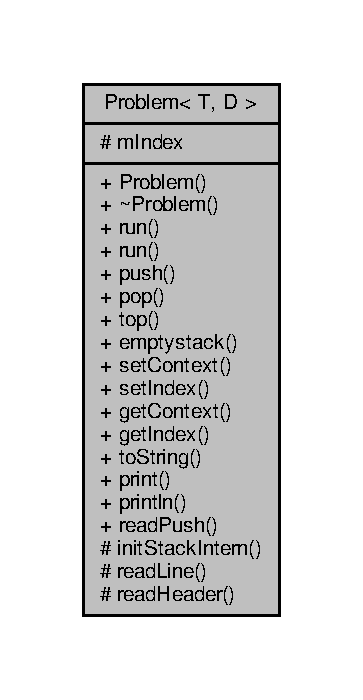
\includegraphics[width=174pt]{class_problem__coll__graph}
\end{center}
\end{figure}
\subsection*{Public Member Functions}
\begin{DoxyCompactItemize}
\item 
{\bfseries Problem} (std\+::string file\+Name)\hypertarget{class_problem_a12573e7fe2b81d50f5c1cdeef3c40aab}{}\label{class_problem_a12573e7fe2b81d50f5c1cdeef3c40aab}

\item 
void {\bfseries run} ()\hypertarget{class_problem_a8ce5fef9d031d039f1108e2c8e37dc0c}{}\label{class_problem_a8ce5fef9d031d039f1108e2c8e37dc0c}

\item 
void {\bfseries run} (int limit)\hypertarget{class_problem_ac005fa3508b7919a0dfe8a27674e1e88}{}\label{class_problem_ac005fa3508b7919a0dfe8a27674e1e88}

\item 
void {\bfseries push} (\hyperlink{class_data}{Data}$<$ T, D $>$ elt)\hypertarget{class_problem_a0646d0ab10243ede1bfd8d20c87ebb21}{}\label{class_problem_a0646d0ab10243ede1bfd8d20c87ebb21}

\item 
\hyperlink{class_data}{Data}$<$ T, D $>$ {\bfseries pop} ()\hypertarget{class_problem_acbf710851a036b2602d32190cdf2ba89}{}\label{class_problem_acbf710851a036b2602d32190cdf2ba89}

\item 
\hyperlink{class_data}{Data}$<$ T, D $>$ {\bfseries top} (int k)\hypertarget{class_problem_aad2184ad1ce770cce1d9008435bb4055}{}\label{class_problem_aad2184ad1ce770cce1d9008435bb4055}

\item 
bool {\bfseries emptystack} ()\hypertarget{class_problem_a8393e40932145b955883cf422091d964}{}\label{class_problem_a8393e40932145b955883cf422091d964}

\item 
void {\bfseries set\+Context} (const T \&context)\hypertarget{class_problem_ad9e49e1c165929877f159f51ce7bd040}{}\label{class_problem_ad9e49e1c165929877f159f51ce7bd040}

\item 
void {\bfseries set\+Index} (int index)\hypertarget{class_problem_a96a72225d5c9a7897551d08646b9c2ae}{}\label{class_problem_a96a72225d5c9a7897551d08646b9c2ae}

\item 
T {\bfseries get\+Context} ()\hypertarget{class_problem_ad863a03e7d0b6f1e1fa8fd1eef9d5b74}{}\label{class_problem_ad863a03e7d0b6f1e1fa8fd1eef9d5b74}

\item 
int {\bfseries get\+Index} ()\hypertarget{class_problem_a09511acd5bec03c7a75bf58d19645a98}{}\label{class_problem_a09511acd5bec03c7a75bf58d19645a98}

\item 
std\+::string {\bfseries to\+String} ()\hypertarget{class_problem_a0557ccf99dec38574270a6385ece70d0}{}\label{class_problem_a0557ccf99dec38574270a6385ece70d0}

\item 
void {\bfseries print} ()\hypertarget{class_problem_a3bbf44cb316faa44afdc351ebdac6a4c}{}\label{class_problem_a3bbf44cb316faa44afdc351ebdac6a4c}

\item 
void {\bfseries println} ()\hypertarget{class_problem_acb9ad1df46781fd0ccfd7aae4c0cbbfa}{}\label{class_problem_acb9ad1df46781fd0ccfd7aae4c0cbbfa}

\item 
void {\bfseries read\+Push} (int iter=1)\hypertarget{class_problem_a7fcfe23395fd9ff931f502a2d7fc7499}{}\label{class_problem_a7fcfe23395fd9ff931f502a2d7fc7499}

\end{DoxyCompactItemize}
\subsection*{Protected Member Functions}
\begin{DoxyCompactItemize}
\item 
void {\bfseries init\+Stack\+Intern} ()\hypertarget{class_problem_a784152fad7b879e224304e666194bc5f}{}\label{class_problem_a784152fad7b879e224304e666194bc5f}

\item 
std\+::vector$<$ std\+::string $>$ {\bfseries read\+Line} ()\hypertarget{class_problem_a8b50749a706399126db45715cdfcd9d9}{}\label{class_problem_a8b50749a706399126db45715cdfcd9d9}

\item 
std\+::vector$<$ std\+::string $>$ {\bfseries read\+Header} ()\hypertarget{class_problem_ab8ccb9161ac36c786522b572a2d70e30}{}\label{class_problem_ab8ccb9161ac36c786522b572a2d70e30}

\end{DoxyCompactItemize}
\subsection*{Protected Attributes}
\begin{DoxyCompactItemize}
\item 
int {\bfseries m\+Index}\hypertarget{class_problem_a3a5c4dbc0ecdff910fe3faf8d78245c6}{}\label{class_problem_a3a5c4dbc0ecdff910fe3faf8d78245c6}

\end{DoxyCompactItemize}
\subsection*{Friends}
\begin{DoxyCompactItemize}
\item 
class {\bfseries Compressed\+Stack$<$ T, D $>$}\hypertarget{class_problem_a0bc563c952d4b72ba232305ab7717bd9}{}\label{class_problem_a0bc563c952d4b72ba232305ab7717bd9}

\item 
class {\bfseries Compare\+Stacks$<$ T, D $>$}\hypertarget{class_problem_aad0b6ceccdc6599793a7e2e5798b59ad}{}\label{class_problem_aad0b6ceccdc6599793a7e2e5798b59ad}

\item 
class {\bfseries Comparison}\hypertarget{class_problem_aef3aa9a02bb7e4bcae2ebd8975a9206d}{}\label{class_problem_aef3aa9a02bb7e4bcae2ebd8975a9206d}

\end{DoxyCompactItemize}


The documentation for this class was generated from the following files\+:\begin{DoxyCompactItemize}
\item 
include/compressed\+Stack.\+hpp\item 
include/problem.\+hpp\end{DoxyCompactItemize}

\hypertarget{class_signature}{}\section{Signature$<$ T, D $>$ Class Template Reference}
\label{class_signature}\index{Signature$<$ T, D $>$@{Signature$<$ T, D $>$}}


Collaboration diagram for Signature$<$ T, D $>$\+:
\nopagebreak
\begin{figure}[H]
\begin{center}
\leavevmode
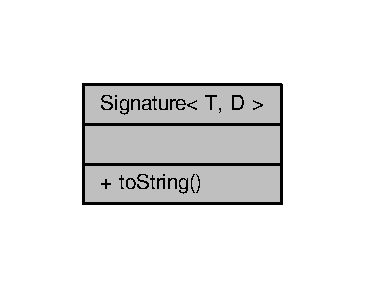
\includegraphics[width=175pt]{class_signature__coll__graph}
\end{center}
\end{figure}
\subsection*{Public Member Functions}
\begin{DoxyCompactItemize}
\item 
std\+::string {\bfseries to\+String} ()\hypertarget{class_signature_a3fab31cb17d15768ad94e697cbe6674d}{}\label{class_signature_a3fab31cb17d15768ad94e697cbe6674d}

\end{DoxyCompactItemize}
\subsection*{Friends}
\begin{DoxyCompactItemize}
\item 
class {\bfseries Component$<$ T, D $>$}\hypertarget{class_signature_a843c2f068a1ab99ce6c9c0e2cc3946c5}{}\label{class_signature_a843c2f068a1ab99ce6c9c0e2cc3946c5}

\item 
class {\bfseries Compressed\+Stack$<$ T, D $>$}\hypertarget{class_signature_a0bc563c952d4b72ba232305ab7717bd9}{}\label{class_signature_a0bc563c952d4b72ba232305ab7717bd9}

\item 
class {\bfseries Normal\+Stack$<$ T, D $>$}\hypertarget{class_signature_a3448f5e6d9366f8729b55e62587568ca}{}\label{class_signature_a3448f5e6d9366f8729b55e62587568ca}

\end{DoxyCompactItemize}


The documentation for this class was generated from the following files\+:\begin{DoxyCompactItemize}
\item 
include/buffer.\+hpp\item 
include/sign.\+hpp\end{DoxyCompactItemize}

\hypertarget{class_stack}{}\section{Stack$<$ T, D $>$ Class Template Reference}
\label{class_stack}\index{Stack$<$ T, D $>$@{Stack$<$ T, D $>$}}


Inheritance diagram for Stack$<$ T, D $>$\+:
\nopagebreak
\begin{figure}[H]
\begin{center}
\leavevmode
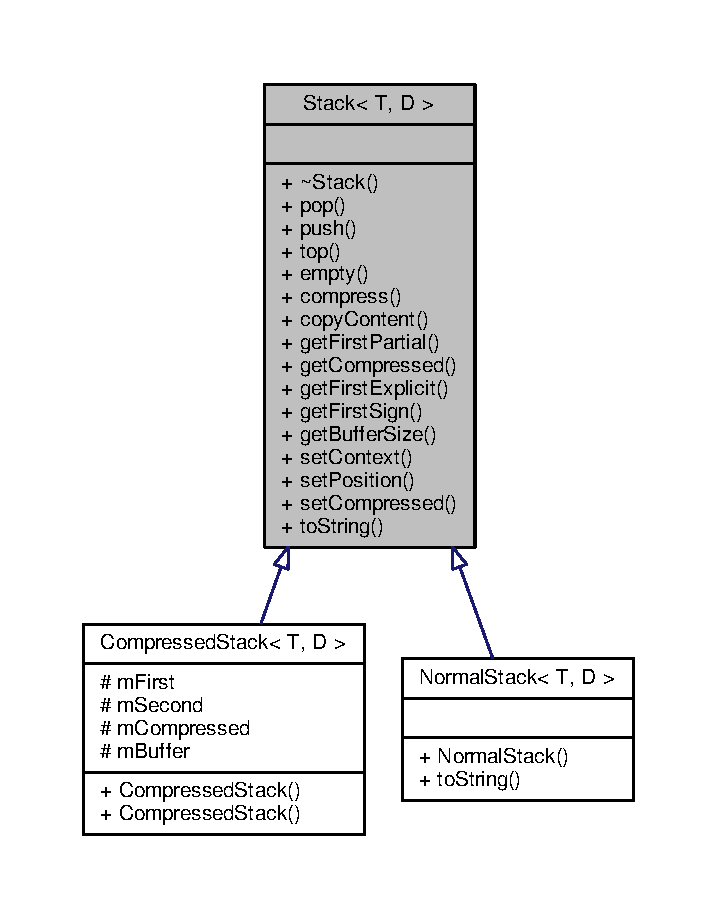
\includegraphics[width=344pt]{class_stack__inherit__graph}
\end{center}
\end{figure}


Collaboration diagram for Stack$<$ T, D $>$\+:
\nopagebreak
\begin{figure}[H]
\begin{center}
\leavevmode
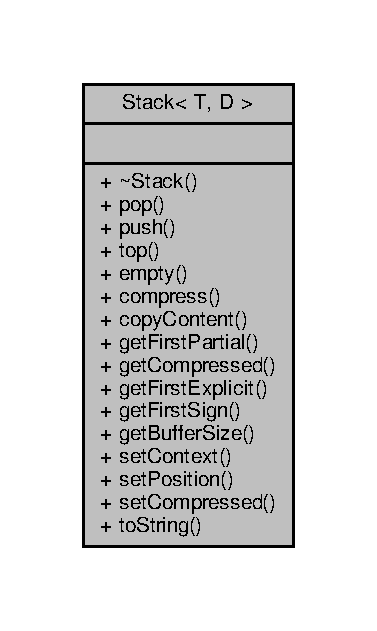
\includegraphics[width=181pt]{class_stack__coll__graph}
\end{center}
\end{figure}
\subsection*{Public Member Functions}
\begin{DoxyCompactItemize}
\item 
virtual \hyperlink{class_data}{Data}$<$ T, D $>$ {\bfseries pop} (\hyperlink{class_problem}{Problem}$<$ T, D $>$ \&problem)=0\hypertarget{class_stack_a9e0581b3b2328bbb8e7771a8023694f9}{}\label{class_stack_a9e0581b3b2328bbb8e7771a8023694f9}

\item 
virtual void {\bfseries push} (const \hyperlink{class_data}{Data}$<$ T, D $>$ \&data)=0\hypertarget{class_stack_a33267fdecb527b595bcd635c37a102b7}{}\label{class_stack_a33267fdecb527b595bcd635c37a102b7}

\item 
virtual \hyperlink{class_data}{Data}$<$ T, D $>$ {\bfseries top} (int k=1)=0\hypertarget{class_stack_a44af4f85e85b9c2aa9a107e4ce4dfb08}{}\label{class_stack_a44af4f85e85b9c2aa9a107e4ce4dfb08}

\item 
virtual bool {\bfseries empty} (int lvl=-\/1, int component=0)=0\hypertarget{class_stack_a3b11a0cb1ec9e2664ac30c03ac1c0d45}{}\label{class_stack_a3b11a0cb1ec9e2664ac30c03ac1c0d45}

\item 
virtual void {\bfseries compress} ()=0\hypertarget{class_stack_a1afc50dff2d38932d1503de659f833a4}{}\label{class_stack_a1afc50dff2d38932d1503de659f833a4}

\item 
virtual void {\bfseries copy\+Content} (\hyperlink{class_compressed_stack}{Compressed\+Stack}$<$ T, D $>$ \&stack)=0\hypertarget{class_stack_aa49e31081a423393dc601defef220f90}{}\label{class_stack_aa49e31081a423393dc601defef220f90}

\item 
virtual Block$<$ T, D $>$ {\bfseries get\+First\+Partial} (int lvl)=0\hypertarget{class_stack_a7c2afc77f96c5a6a28b42e90cb6639b7}{}\label{class_stack_a7c2afc77f96c5a6a28b42e90cb6639b7}

\item 
virtual Block$<$ T, D $>$ {\bfseries get\+Compressed} ()=0\hypertarget{class_stack_a0cc1315782196cc83ee04595f1c10115}{}\label{class_stack_a0cc1315782196cc83ee04595f1c10115}

\item 
virtual Explicit\+Pointer$<$ T, D $>$ {\bfseries get\+First\+Explicit} ()=0\hypertarget{class_stack_a01d1ca3a7216b2ac911b1702cfe8b2a2}{}\label{class_stack_a01d1ca3a7216b2ac911b1702cfe8b2a2}

\item 
virtual \hyperlink{class_signature}{Signature}$<$ T, D $>$ {\bfseries get\+First\+Sign} ()=0\hypertarget{class_stack_ad270abee82575fc6644b84381c0d77b8}{}\label{class_stack_ad270abee82575fc6644b84381c0d77b8}

\item 
virtual int {\bfseries get\+Buffer\+Size} ()=0\hypertarget{class_stack_ab9758df4a9908c9ab2e55ada2adeed44}{}\label{class_stack_ab9758df4a9908c9ab2e55ada2adeed44}

\item 
virtual void {\bfseries set\+Context} (std\+::shared\+\_\+ptr$<$ T $>$ context)=0\hypertarget{class_stack_a115dceb34061f3f85a9690487105e0d4}{}\label{class_stack_a115dceb34061f3f85a9690487105e0d4}

\item 
virtual void {\bfseries set\+Position} (std\+::streampos position)=0\hypertarget{class_stack_a709f0cda4f86650dc32b5dfbd732631b}{}\label{class_stack_a709f0cda4f86650dc32b5dfbd732631b}

\item 
virtual void {\bfseries set\+Compressed} (Block$<$ T, D $>$ block)=0\hypertarget{class_stack_aad51cfcdcabb79dd0ca3af419b482ecd}{}\label{class_stack_aad51cfcdcabb79dd0ca3af419b482ecd}

\item 
virtual std\+::string {\bfseries to\+String} ()=0\hypertarget{class_stack_a0fd2d1fca9cf1909ee73e930150f753d}{}\label{class_stack_a0fd2d1fca9cf1909ee73e930150f753d}

\end{DoxyCompactItemize}


The documentation for this class was generated from the following file\+:\begin{DoxyCompactItemize}
\item 
include/stack.\+hpp\end{DoxyCompactItemize}

%--- End generated contents ---

% Index
\backmatter
\newpage
\phantomsection
\clearemptydoublepage
\addcontentsline{toc}{chapter}{Index}
\printindex

\end{document}
